\documentclass[letterpaper, onecolumn,10pt]{IEEEtran}

\usepackage{graphicx}
\usepackage{amssymb}
\usepackage{amsmath}
\usepackage{amsthm}

\usepackage{alltt}
\usepackage{float}
\usepackage{color}
\usepackage{url}
\usepackage{listings}
\usepackage{ifthen}


\usepackage[TABBOTCAP, tight]{}

\usepackage{geometry}
\geometry{textheight=8.5in, textwidth=6in}

%random comment

\newcommand{\cred}[1]{{\color{red}#1}}
\newcommand{\cblue}[1]{{\color{blue}#1}}

\usepackage{hyperref}
\usepackage{geometry}
\usepackage{caption}
\usepackage{url}
\usepackage{natbib}

\begin{document}
    \begin{titlepage}
    \newcommand{\HRule}{\rule{\linewidth}{0.5mm}}
    \center
    \textsc{\Large Oregon State University}\\[1.5cm]
    \textsc{\Large ST 314}\\[0.5cm]
    \textsc{\Large Summer 2019}\\[0.5cm]
    \HRule \\[0.4cm]
    { \huge \bfseries Data Analysis Five}\\[0.4cm] % Title of your document
    \HRule \\[1.5cm]
    \begin{minipage}{0.4\textwidth}
        \begin{flushleft} \large
        \emph{Author:}\\
        Thomas Noelcke
        \end{flushleft}
    \end{minipage}
    \begin{minipage}{0.4\textwidth}
        \begin{flushright} \large
        \emph{Instructor:} \\
        Katie Jager\\
        \end{flushright}
    \end{minipage}\\[2cm]
		\end{titlepage}
        
        \section{Part 1}
            \subsection{}
            %include boxplot here
            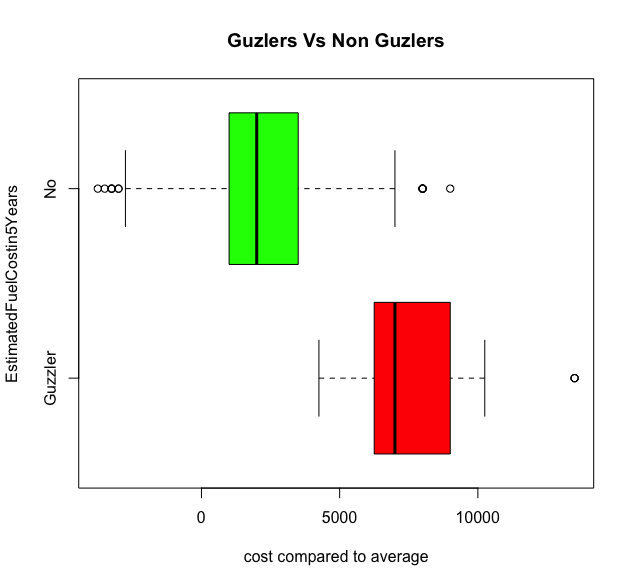
\includegraphics[width=\textwidth]{week5/boxplot1.png}
            
            \subsection{}
            The distribution of the data for non guzzlers vs guzzlers does suggest that the non guzzlers on average burn less fuel than guzzlers. This is illustrated by the fact that the first quartile of the guzzlers is out side the 3rd quartile of the non guzzlers. The average consumption of the non guzzlers is also much lower than the the guzzlers. I do find it interesting that there are non guzzlers that consume fuel such that maybe they should be guzzlers.\\
            
            \subsection{}
            \begin{table}[ht]
                \centering
                \begin{tabular}{c|c|c|c}
                     & Mean & Standard Deviation & Sample Size\\
                     GUZZLER & 7861.111 & 2202.326 & 36\\
                     NON-GUZZLER & 2202.326 & 2111.156 & 860\\
                \end{tabular}
            \end{table}
            
            \subsection{}
            Guzzlers are entirely composed of luxury cars and super cars. These type of cars tend to be high performance cars with large engines.\\
            
            
        \section{Part 2}
            \subsection{Calculate}
                \subsubsection{}
                    Shown Below is the Calculation of the test statistic:
                    
                    \[
                        t=\dfrac{(X_bar1 - X_bar2)-\sigma}{\sqrt{\dfrac{s^2_1}{n_1} + \dfrac{s^2_2}{n_2}}}
                    \]
                    \[
                        =\dfrac{(7861.111-2202.326) - 0}{\sqrt{\dfrac{2170.784^2}{36} + \dfrac{2202.326^2}{860}}} =~15.3143
                    \]
                \subsection{}
                    I'm choosing to use conservative degrees of freedom. In this case the degrees of freedom are as follows:
                    
                    \[
                        min(n_1 - 1, n_2 -1) = 35
                    \]
                \subsection{}
                    The p Value for our test statistic will be approximately 0. If we look at the t table we will find that the nearest value that matches up is 99.9 at 35 degrees of freedom is only around 3.5.\\
                
                \subsection{}
                    Shown below is my calculation for the 99\% confidence interval.
                    
                    \[
                        (X_bar1 - X_bar2) \pm t^* \sqrt{\dfrac{s^2_1}{n_1}+\dfrac{s^2_2}{n_2}}
                    \]
                    \[
                        = (7861.111 - 2202.326) \pm  2.7238 * \sqrt{\dfrac{2170.784^2}{36}+\dfrac{2202.784^2}{860}} = [4652.54, 6664.8]
                    \]
                \subsection{}
                    Stats From R:
                    \begin{table}[ht]
                        \centering
                        \begin{tabular}{c|c}
                            t statistic & 15.34\\
                            p-Value & 2.2e-16\\
                            99\% Interval & [4658.28, 6659.30]\\
                        \end{tabular}
                    \end{table}
                    
                    The values that R Calculated and the values that I found by hand are similar however there are some differences. The differences that you see are due to the fact that I chose the conservative estimation for degrees of freedom rather than the Satterwaite method.\\
            
            \subsection{Conclude}
                \subsubsection{}
                There is convincing evidence that the difference between the Guzzlers and non Guzzlers is not zero.\\
                
                \subsubsection{}
		        We reject the null hypothesis in this case with a test statistic of 15.34 and a p-value of 2.2e-16.
		        
		        \subsubsection{}
		        On average Guzzlers cost \$5658.79 to operate over 5 years when compared to non guzzlers with a 99\% confidence interval of 4658.28 to 6659.30.\\ 
		\end{document}